\section{Lessons Learned Perspective}
\subsection{Evolution and Refactoring}
% Subjects:
% -From one BIG FILE to a whole folder organization.
% -Python template to Go template. (rendering front-end with go)
% -Go template to React.
% -Database migration (Big challenge to refactor from the old version)
% -Nothing more for "evolution from the old system" 
% \\
The successive transitions of our system from one huge Python file to Go (Release v2.0.0\footnote{Release v2.0.0 found here: 
\href{https://github.com/DevOps-Ben11/minitwit/releases/tag/v2.0.0}{github.com/DevOps-Ben11/minitwit/releases/tag/v2.0.0}}.) followed by a smart folder structure (Release v3.0.0\footnote{Release v3.0.0 found here: 
\href{https://github.com/DevOps-Ben11/minitwit/releases/tag/v3.0.0}{github.com/DevOps-Ben11/minitwit/releases/tag/v3.0.0}}) and ending up with a Go-React stack (Release v5.0.0\footnote{Release v5.0.0 found here:
\href{https://github.com/DevOps-Ben11/minitwit/releases/tag/v5.0.0}{github.com/DevOps-Ben11/minitwit/releases/tag/v5.0.0}}) were significant architectural changes. The changes were accompanied by their loads of issues like how to swap from Python templates to Go templates and how to manage user connection and disconnection with React for instance. 
\\
\\
These changes enhanced the scalability and maintainability of the system and show how organizing front-end and back-end logic strategically can help us improve our system. The issues that appeared later were easily fixed thanks to our strategic organizations like for instances high response time (Issue \char"0023 38\footnote{Issue \#38 found here: 
\url{https://github.com/DevOps-Ben11/minitwit/issues/38}}) and security (Issue \char"0023 36\footnote{Issue \#36 found here:
\url{https://github.com/DevOps-Ben11/minitwit/issues/36}}).

\subsection{Operation}
% subjects: 
% -CI/CD pipelines
% -Docker swarm was the big challenge.
% -IaC from vagrant to terraform
% \\
One of the first issues we encountered during operations was the server downtime during system updates. Indeed we were determined to keep the simulation errors as low as possible to keep the users satisfied. 
\\
\\
After setting up the CD pipeline, we agreed that pushes to main should be protected and strategically operated. Before the implementation of docker swarm and the blue-green strategy (Release v5.0.5\footnote{Release v5.0.5 found here: 
\href{https://github.com/DevOps-Ben11/minitwit/releases/tag/v5.0.5}{github.com/DevOps-Ben11/minitwit/releases/tag/v5.0.5}}), we tried to ensure that merges to main would not crash the production. This was done by performing a great amount of testing before approving the pull requests. Major releases called for meetings between group members, to ensure that we all understood and were satisfied with the new features. This organization taught us to carefully prepare changes that happen on the production environment. Lastly, if feasible, tests on new features were performed on a sandbox environment. 

% Setting up Docker Swarm and integrating Prometheus, Grafana and Loki for monitoring and logging was a particularly challenging and time-consuming processes. This process involved extensive local testing and the discovery of new tools. For instant Docker Swarm Visualizer helped us to better understand the swarm's behaviour.

\subsection{Maintenance}
% subjects: 
% -Loggings and Metrics is maintenance, issues: making it works in docker swarm, storage solutions, usage issue \#15.
% -Ssh connections to change stuff is maintenance, issues: subjects to human error.
% \\
In the Regional Latency diagram of Figure \ref{fig:Indexing latency problem}, we observe that the server's response time was increasing as the SQLite database was getting filled by the simulation requests. We noticed this issue on the Digital Ocean dashboard and that it was getting critical as some simulation requests got timed out. We worked on this issue as soon as we noticed it and fixed it (Release v3.2.10\footnote{Release v3.2.10 found here: 
\href{https://github.com/DevOps-Ben11/minitwit/releases/tag/v3.2.10}{github.com/DevOps-Ben11/minitwit/releases/tag/v3.2.10}}).
\\
\\
As we can see in the upper diagram of Figure \ref{fig:Indexing latency problem}, benefits were instant and the latency decreased drastically, allowing our system to continue handling the simulation. 
\begin{figure}[H]
    \centering
    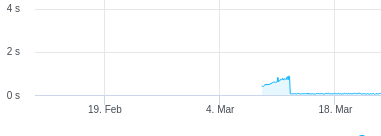
\includegraphics[scale=.9]{img/indexing_latency_3.png}
    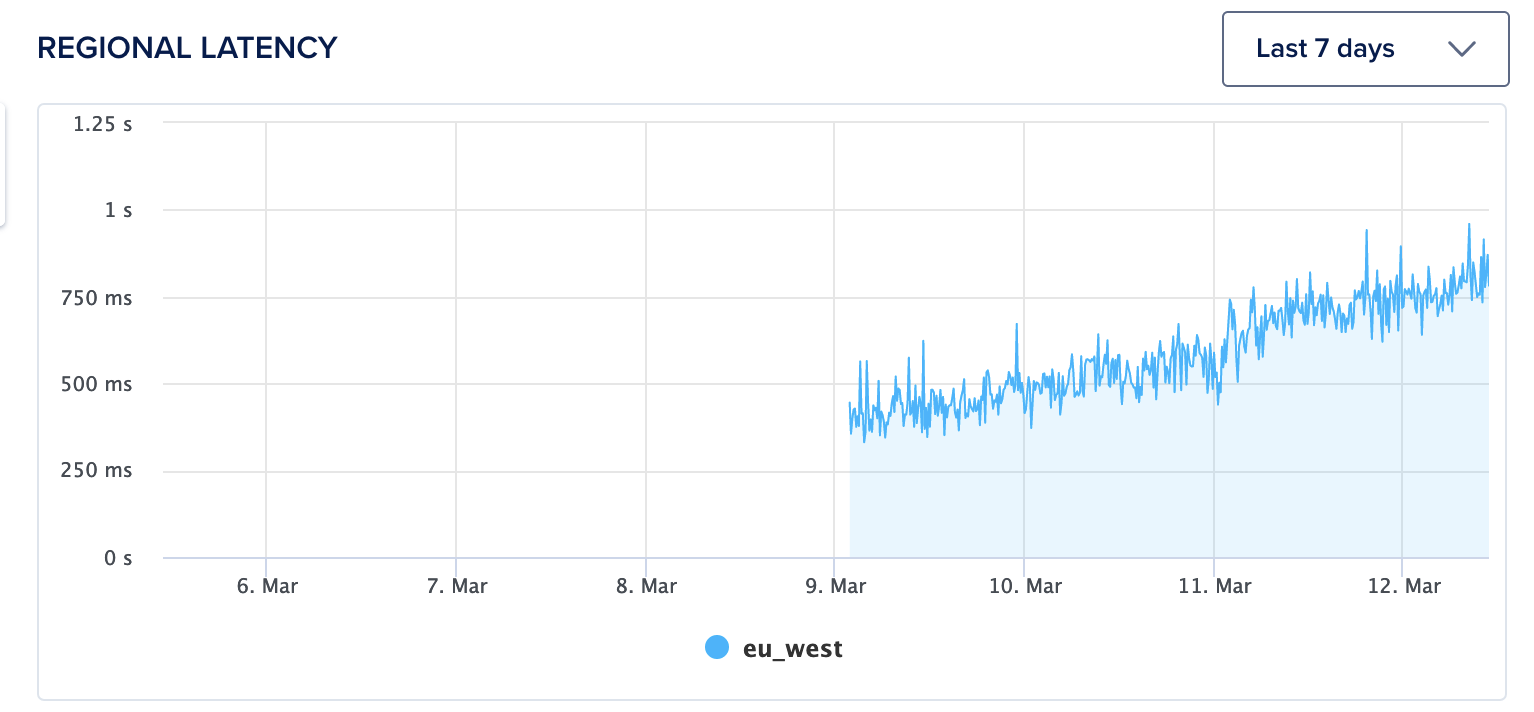
\includegraphics[scale=.4]{img/indexing_Latency_2.png}
    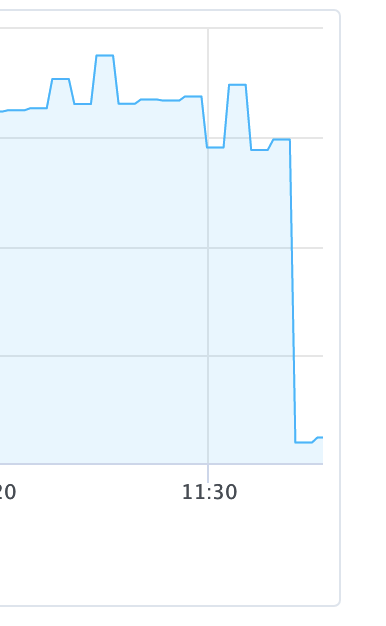
\includegraphics[scale=.4]{img/indexing_Latency_1.png}
    \caption{Images showing the latency of Minitwit}
    \label{fig:Indexing latency problem}
\end{figure}


Ensuring continuous improvements to Minitwit was challenging and required maintenance on live servers. Initially and during the whole process, many tasks required manual SSH connections to our droplets. Even though, different operational tools, such as Vagrant, helped ensure a more systematic and seamless interaction with the server. 
\\
\\
These frequent SSH connections to modify for instance environment variables and to manage the system were necessary but also time-consuming and prone to human error, often leading to intense situation to reduce servers downtime.
\\
\\
More advanced automating deployment and maintenance processes have reduced the need for manual interventions, decreasing the risk of human error and improving efficiency.


